\chapter{System Description}
This chapter will give a description of the VR sketch-based modelling software, named SketchMeshVR, that was developed as part of this thesis. The software aims to provide users with a simple and intuitive sketch-based 3D modelling tool within a VR environment. Specifically the software is developed for use with the Oculus Rift including one Touch controller. Compared to the VR modelling software that was discussed in Section ~\ref{}\todo{insert section 3d modelling in vr} our system provides a novel method for creating 3D models. Whereas the existing modelling tools utilize volumetric brushes or predefined 3D shapes, our tool lets the user define the outline of a 3D shape and then fills in the inside of the outline. 

\section{Algorithms}
Algorithmically, SketchMeshVR largely follows FiberMesh by \cite{Nealen2007}. Similar to FiberMesh, users can draw strokes that define the 3D mesh surface, and these drawn strokes stay on the model surface to later function as deformation handles. Users can create an initial mesh, cut parts of the mesh, create extrusions, add and remove additional control curves and deform control curves on the mesh. Unlike in FiberMesh, SketchMeshVR does not give users the option to choose between smooth and sharp constraint curves and instead all curves are treated as smooth. The functionality to create tunnels through meshes is also not present in SketchMeshVR.  

SketchMeshVR is built inside the framework of libigl \cite{Jacobson2017} and uses Oculus C++ SDK in order to display everything on the Oculus Rift. The standard overlay menu that is included in libigl is disabled since the concept of overlays does not port well to the VR setting. Overlays are displayed too close to the eye making it very difficult for the eye to focus on them, which results in a highly unpleasant user experience. 

The system is multithreaded such that the VR display keeps on being updated while the mesh computations are being executed. When multithreading is not enabled the screen will freeze during the mesh computations, and therefore will stop updating when the user moves his head, breaking immersion and likely inducing motion sickness. 

Due to the direct availability of the actual 3D coordinates, some changes were made in comparison to the non-VR version. 
Whereas the non-VR version in drawing mode starts by converting mouse positions to screen coordinates and then unprojects these to 3D coordinates with a z-value of 0, SketchMeshVR takes the actual 3D coordinates and only projects them to 2D to allow triangulation. 
In the non-VR case, adding control curves on the mesh and later removing them is done by unprojecting the screen coordinates onto the mesh in order to get 3D positions and decide where the user wanted to add/remove a curve. In VR, instead of unprojecting the screen coordinates of the hand or taking the direct hand coordinates, we cast a ray from the hand position in the direction that the controller is being held. This intersection between this ray and the mesh is then used as the final 3D position for adding/removal.
When cutting in the non-VR program, the drawn stroke is interpreted purely in 2D. In order to create a loop on the front and back of the mesh surface, it is checked what edges are crossed (in 2D) by a line segment between two consecutive stroke points. Since the same 2D points are used for creating a surface path on the backside of the mesh, this results in perpendicular cuts (meaning that the "cutting knife" always goes perpendicular through the screen, and never at an angle). On the other hand, when cutting in VR we take the coordinates of both the first and second intersection between the cutting ray and the mesh. By doing this, we enable the possibility for the user to cut the mesh diagonally. In order to check which edges are crossed by the stroke segments, we find intersections between edges and the plane that is formed by the two points that make up the stroke segment and the position of the hand at the time of drawing that stroke segment. If an edge is intersected within its range, we know that the stroke segment crosses that edge. The surface path for the extrusion base is created in a similar fashion, except that only the first hit between ray and mesh is used. One problem that arises due to the fact that we're using 3D intersection points between the cutting ray and the mesh, is that we cannot easily derive the start and end points of the cutting stroke. These points are the final point outside of the mesh before we start drawing on top of the mesh and the first point outside of the mesh after drawing on top of the mesh respectively. \todo{probably include a drawing of this} We need these points in order to be able to find the mesh boundary edges that we need to cross to wrap the surface path around to the backside of the mesh. As mentioned before, in the non-VR case we simply use 2D coordinates based off the screen coordinates of the mouse pointer. In VR we cannot take the position of the controller as the user is likely cutting from a distance. What we've done in order to determine the start and end point is storing the controller position and direction for every sampled point that does not intersect the mesh. Then when the user releases the controller buttons after drawing  the cut stroke, we take these positions and directions and along these rays find the two points that are closest to the first and last point drawn onto the mesh. Under normal circumstances this will then give the two points outside of the mesh that are closest to the first and final cutting stroke points on the mesh. This method does however somewhat restrict the user in their freedom on how to draw the cut stroke. If the user holds his hand close to the mesh when starting the cut stroke, it is possible that the closest point to the initial on-mesh point actually is projected onto the mesh. This will make it impossible to create a looped surface path over the mesh. If this happens, a beep will sound and the cut stroke will be shown in black, allowing the user to try again.  \todo{probably include image}

Drawing the extrusion silhouette in VR is significantly different from the way it is done in non-VR. When defining the silhouette stroke in non-VR, the user first has to rotate the mesh such that it is looked at from a side view. Only then can the user sensefully specify the shape and depth of the extrusion silhouette, since we cannot gain any depth information from a frontal view. In VR on the other hand, we know the actual 3D positions of the controller and can therefore directly specify the extrusion silhouette in the frontal view. If the user prefers to do this from a side view instead (to get additional visual feedback about the silhouette depth on top of the tactile feedback), this is also possible.
Finally \todo{pull}

\section{User Interface}
For the user interface in virtual reality it was important to keep the controls for all actions very intuitive. Unlike the VR 3D modelling programs that were discussed in the previous work section\todo{put a ref to the specific section here}, SketchMeshVR does not have any menus in its interface. Instead all functionality in the program can be used with just the right Touch controller (in future versions the user should be able to choose whether to use the left or right controller as the primary one). To simplify orientating the user's hand in the scene, a sphere is displayed at the location of the right Touch controller, together with a ray from the hand following the orientation of the controller. When the user is in draw or pull mode or is drawing the extrusion silhouette, the ray disappears and only the hand sphere shows. This is done in order to emphasize that the actual position of the hand is used to draw a stroke, instead of the intersection points of the ray and mesh.

Compared to drawing strokes with a mouse on a PC screen (which happens purely in a 2D plane), drawing strokes in virtual reality with the Oculus Touch controller allows the user to draw strokes directly in 3D. In SketchMeshVR we made use of this advantage whenever possible. \todo{TEST DRAWING IN YZ PLANE (BUT NOT FULLY PERPENDICULAR)} However, when the user draws the stroke that is used to create the initial mesh, the software does assume that the stroke is drawn mostly on the plane that the user is looking at. This is due to the fact that the drawn points will be projected to this 2D plane before they are triangulated. Subsequent cutting or extrusion operations do not have to be made in the plane that is being viewed, as for these actions the actual 3D positions of the drawn points are used. 

\todo{position touch controller image}
To create an initial mesh, the user has to simultaneously press and hold the grip and trigger buttons while drawing a stroke in the air and subsequently release both when the stroke is finished. If the drawn stroke results in a non-edge manifold mesh (for example if the stroke intersects itself), a beep will sound and the stroke is displayed in black. Otherwise the created mesh will be shown, with the originally drawn stroke overlayed. 

In order to deform the mesh, a user can drag on all present mesh curves. The user can toggle between drawing and deformation mode by pressing the B button. Upon startup draw mode is selected. To perform the dragging, the user has to simultaneously press and hold down the grip and trigger buttons while his hand is close to the curve vertex that he wants to pull to a new position. Then while still pressing the grip and trigger buttons, the user needs to move his hand to the desired new position, and release both buttons when the desired result is achieved. The new vertex position is interpreted directly as the 3D position of the Touch controller, therefore also allowing deformation outside of the viewing plane (as compared to the non-VR version, which only allows in-plane deformation). 

The combination of grip and trigger buttons was chosen for these actions as they most resemble the feeling of holding a pencil and grabbing something in order to pull on it. 

To add extra control curves to an existing mesh, the user has to press and hold the trigger button while drawing the stroke onto the mesh. All points that are outside of the mesh will be ignored and will not be added to the control curve. 

In order to remove control curves (all except for the curve that created the initial mesh), the user can toggle from stroke adding mode to stroke removal mode by pressing down the right thumbstick. Upon startup the stroke adding mode is selected. 
\todo{say something about ray mesh intersection for both add and remove}

We decided to map the trigger button to the functions of adding and removing control curves since this feels like a natural way to select objects (removal) and to highlight areas (addition).

Finally with the B button the user can switch between cut and extrusion modes. Upon startup the toggle is set to cutting mode, which allows the user to cut off parts of the existing mesh. To make a cut the user has to first point the laser ray to somewhere outside of the mesh, and then while holding down the grip button draw the cutting stroke over the mesh and finally releasing somewhere outside of the mesh again. In order to minimize unwanted behaviour, the user's hand should be a distance of approximately the mesh diagonal away from the mesh when performing a cut action. If anything went wrong during the cutting procedure, the drawn stroke will show on the mesh in black and a beep will sound. 
When in extrusion mode, the user has to start on the mesh and then while pressing the grip button has to draw the extrusion base on the mesh and release the button when the stroke is complete. Just like in the control curve addition mode, any points that are drawn outside of the mesh will be ignored. To ensure a correct functioning of the algorithm, the drawn base stroke has to have at least one vertex on its interior. Then to complete the extrusion, the user has to draw the extrusion silhouette stroke that will define the height of the extrusion. When drawing this stroke, the user has to press and hold the grip button again but this time the actual position of the Touch controller will be used instead of the ray-mesh intersection point. Releasing the grip button will start the extrusion computations.

When pressing only the grip button, the hand often naturally assumes a position that resembles the way we symbolize pistols with our hands. Intuitively this maps to the concept of shooting a laser ray from your hand, which would be a sensible tool to cut a mesh with. For the case of extrusion we can argue something similar, as part of the mesh topology is also cut away. For this reason the grip button was mapped to the cut and extrude modes.

\begin{figure}[!h]
    \centering
    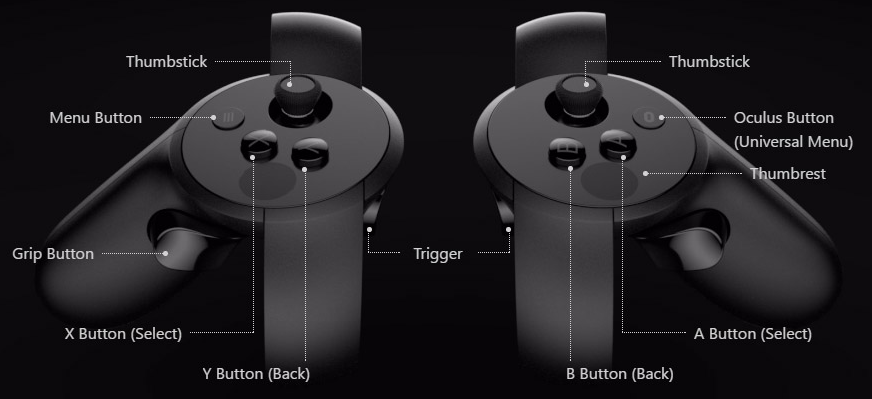
\includegraphics[width=0.7260\linewidth]{figures/touch_controllers}\\
    \caption[Oculus Touch controllers]{Button layout of the Oculus Touch controllers.
      \label{fig:touch_controller}}
\end{figure}


\begin{table}
    \centering
    \ra{1.1}
    \begin{tabular}{lp{0.4\linewidth}}
    \toprule
    \emph{Quant.} & \emph{Ingredient}\\
    \midrule
		200g &Wei{\ss}mehl\\
		1/4  &Packung Frischhefe\\
		4EL  &lauwarme Milch\\
		4EL  &�l\\
		1TL  &Zucker\\
		1TL  &Salz\\
		&lauwarmes Wasser\\
    \bottomrule
    \end{tabular}
    \caption[Flammkuchenteig]{Flammkuchenteig. The ingredients have to be carefully chosen.\label{tab:mytable}}
\end{table}


